\section{Auswertung}
\label{sec:Auswertung}

\subsection{Messung der Zählrate und der Energie von Alpha-Strahlung}
In Tabelle \ref{tab:Mess1} sind die gemessene Zählrate und der Channel bei variierendem Druck gemessen worden.
Dabei beträgt die Entfernung zwischen Detektor und Präparat $\qty{2.3}{\centi\meter}$. Eine Messvorgang dauert 2 Minuten.
Die Channel sind ein indirektes Maß für die Energie. Es wird angenommen, dass die Alpha-Teilchen bei
einem Druck von $\qty{0}{\milli\bar}$ eine maximale Energie von $\qty{4}{\mega\electronvolt}$ besitzen.
Damit lässt sich bei der Messung aus Tabelle \ref{tab:Mess1} der Channel 816 der Energie $\qty{4}{\mega\electronvolt}$
zuordnen. Die anderen Channel folgen dieser Zuordnung linear. Also Channel 408 entspricht
einer Energie von $\qty{2}{\mega\electronvolt}$.
Damit ergibt sich für die Energie
\begin{equation}
  E=\frac{\text{Channel}}{816}\cdot \qty{4}{\mega\electronvolt}.
  \label{eq:En1}
\end{equation}
Genauso lässt sich mit Gleichung \eqref{eq:ptox} dem Druck eine effektive Entfernung zum Präperat
bei Normaldruck bestimmen. Dabei ist $x_0=\qty{2.3}{\centi\meter}$.
Die korrespondierenden Längen und Entfernungen sind ebenfalls in Tabelle \ref{tab:Mess1} angegeben.
\begin{table}[H]
  \centering
  \caption{Messreihe 1 bei einer Entfernung von $\qty{2.3}{\centi\meter}$ und nach 2 Minuten}
  \label{tab:Mess1}
  \begin{tabular}{S[table-format=4] S[table-format=3] S[table-format=5] S[table-format=1.2] S[table-format=1.2]}
    \toprule
      {Druck/mbar} & {Channel} & {Zählrate/2min}&{effektive Entfernung/$\unit{\centi\meter}$} &{Energie in MeV}\\
    \midrule
    0 & 816 & 84290 & 0.00 & 4.00 \\
    50 & 768 & 83234 & 0.11 & 3.76 \\
    100 & 751 & 82737 & 0.23 & 3.68 \\
    150 & 731 & 82099 & 0.34 & 3.58 \\
    200 & 711 & 82005 & 0.45 & 3.49 \\
    250 & 679 & 80538 & 0.57 & 3.33 \\
    300 & 640 & 80144 & 0.68 & 3.14 \\
    350 & 632 & 79189 & 0.80 & 3.10 \\
    400 & 647 & 78107 & 0.91 & 3.17 \\
    450 & 608 & 77703 & 1.02 & 2.98 \\
    500 & 563 & 76030 & 1.14 & 2.76 \\
    550 & 542 & 75554 & 1.25 & 2.66 \\
    600 & 511 & 74284 & 1.36 & 2.50 \\
    650 & 476 & 73075 & 1.48 & 2.33 \\
    700 & 448 & 71075 & 1.59 & 2.20 \\
    750 & 416 & 69127 & 1.71 & 2.04 \\
    800 & 399 & 66378 & 1.82 & 1.96 \\
    850 & 352 & 60823 & 1.93 & 1.73 \\
    900 & 295 & 49233 & 2.05 & 1.45 \\
    950 & 286 & 41287 & 2.16 & 1.40 \\
    1000 & 271 & 26338 & 2.27 & 1.33 \\
      \bottomrule
  \end{tabular}
\end{table}
\noindent Zur besseren Einordnung wird noch eine zweite Messreihe als Vergleich aufgenommen.
Die Ergebnisse sind in Tabelle \ref{tab:Mess2} aufgeführt. Die zweite Messreihe ist bei einer größeren
Distanz zwischen Detektor und Präparat von $\qty{3.2}{\centi\meter}$ gemessen worden.
In dieser Messreihe sind im Vakuum die meisten Detektionen bei Channel 815 aufgetreten.
Damit ergeben sich die dazugehörigen Energien durch
\begin{equation}
  E=\frac{\text{Channel}}{815}\cdot \qty{4}{\mega\electronvolt}.
  \label{eq:En2}
\end{equation} 
Die effektiven Entfernungen ergeben sich bei der 2. Messreihe erneut nach Gleichung \eqref{eq:ptox}.
Die Normaldruckentfernung $x_0$ beträgt dabei $\qty{3.2}{\centi\meter}$.
\begin{table}[H]
  \centering
  \caption{Messreihe 2 bei einer Entfernung von $\qty{3.2}{\centi\meter}$ und nach 2 Minuten}
  \label{tab:Mess2}
  \begin{tabular}{S[table-format=4] S[table-format=3] S[table-format=5] S[table-format=1.2] S[table-format=1.2]}
    \toprule
      {Druck/mbar} & {Channel} & {Zählrate}&{effektive Entfernung/$\unit{\centi\meter}$} &{Energie in MeV}\\
    \midrule
          0 & 815 & 54534 & 0.00 & 4.00 \\
      50 & 768 & 54488 & 0.16 & 3.77 \\
      100 & 736 & 53859 & 0.32 & 3.61 \\
      150 & 704 & 52402 & 0.47 & 3.46 \\
      200 & 687 & 52286 & 0.63 & 3.37 \\
      250 & 643 & 51419 & 0.79 & 3.16 \\
      300 & 591 & 50703 & 0.95 & 2.90 \\
      350 & 576 & 49985 & 1.11 & 2.83 \\
      400 & 560 & 49203 & 1.26 & 2.75 \\
      450 & 531 & 48215 & 1.42 & 2.61 \\
      500 & 480 & 46999 & 1.58 & 2.36 \\
      550 & 439 & 45683 & 1.74 & 2.15 \\
      600 & 399 & 43407 & 1.89 & 1.96 \\
      650 & 371 & 40089 & 2.05 & 1.82 \\
      700 & 300 & 33582 & 2.21 & 1.47 \\
      750 & 276 & 15318 & 2.37 & 1.35 \\
      800 & 267 & 5750 & 2.53 & 1.31 \\
      850 & 267 & 501 & 2.69 & 1.31 \\
      \bottomrule
  \end{tabular}
\end{table}
\subsubsection{Energieverlust von Alpha-Strahlung}
Im Folgenden soll ermittelt werden, wie viel Energie die Alpha-Teilchen pro Wegeinheit
an die umgebende Luft abgeben. Dafür wird jedem Druck eine effektive Entfernung zum Detektor zugeordnet.
Ein Alpha-Teilchen trifft bei halben Atmosphärendruck auf die Hälfte der Luftmoleküle. Damit interagiert
das Teilchen mit genauso vielen Molekülen, wie wenn die Distanz halb so groß ist.
Daher kann die Abhängigkeit zwischen Energie und Weg direkt aus der Abhängigkeit zwischen detektierter Energie
der Alpha-Teilchen und dem eingestellten Druck ermittelt werden.
In Abbildung \ref{fig:Energie1} ist diese Abhängigkeit bei einer festen Distanz von $\qty{2.3}{\centi\meter}$ 
dargestellt. Es lässt sich ein lineare Zusammenhang mit einer Steigung von $\frac{\symup{d}E}{\symup{d}p}=\qty{-2.65}{\mega\electronvolt\per\bar}$
feststellen. Die lineare Regression ist mit der Funktion Polyfit aus der Numpy-Bibliothek erstellt worden \cite{numpy}.
Durch den linearen Zusammenhang zwischen Druck und effektiver Reichweite \eqref{eq:ptox}, ergibt sich ein konstanter Energieverlust der Alpha-Teilchen
von $\frac{\symup{d}E}{\symup{d}x}=\qty{-1.17}{\mega\electronvolt\per\centi\meter}$
\begin{figure}[H]
  \centering
  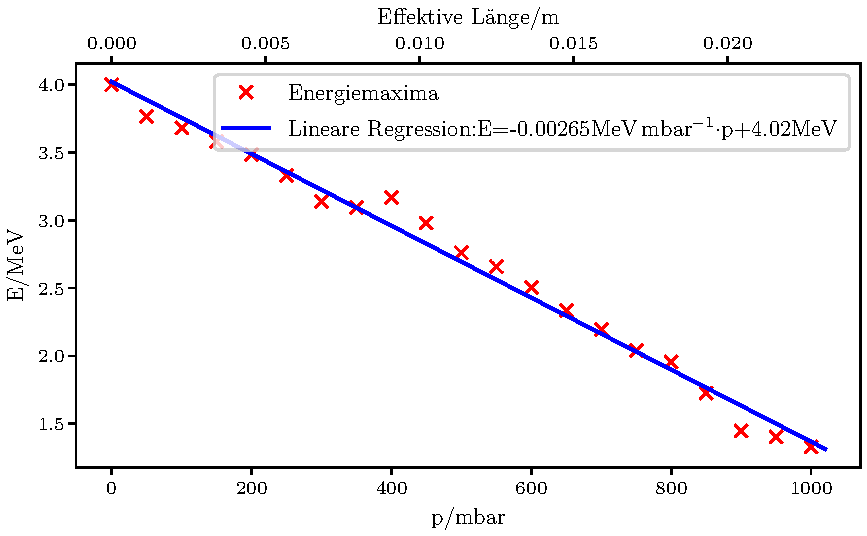
\includegraphics{Energiemaxima1.pdf}
  \caption{Energie von Alpha-Strahlung bei $\qty{2.3}{\centi\meter}$ Entfernung}
  \label{fig:Energie1}
\end{figure}
\noindent Der gleiche Auswertungsprozess wird nun für die zweite Messreihe bei einer Entfernung von $\qty{3.2}{\centi\meter}$
wiederholt. Die Datenpunkte und die lineare Regression sind in Abbildung \ref{fig:Energie2} abgebildet.
Die Änderung der Energie pro Centimeter ergibt sich zu $\frac{\symup{d}E}{\symup{d}x}=\qty{-1.05}{\mega\electronvolt\per\centi\meter}$.
\begin{figure}[H]
  \centering
  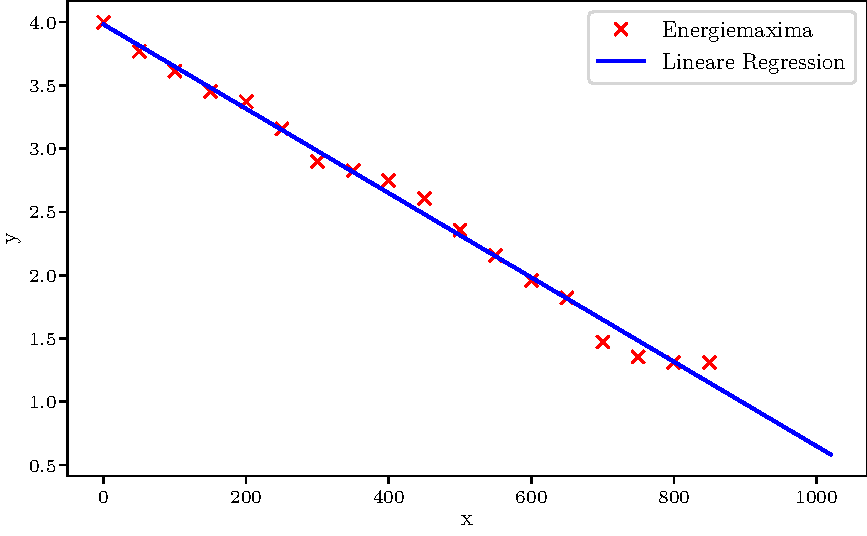
\includegraphics{Energiemaxima2.pdf}
  \caption{Energie von Alpha-Strahlung bei $\qty{3.2}{\centi\meter}$ Entfernung}
  \label{fig:Energie2}
\end{figure}

\subsubsection{Bestimmung der mittleren Reichweite von Alpha-Strahlung in Luft}
Die mittlere Reichweite von Alpha-Strahlung definiert sich dadurch, dass nur die Hälfte der emittierten Alpha-Teilchen
detektiert werden. In Abbildung \ref{fig:Rate1} sind die gemessenen Zählraten den effektiven Entfernungen
zugeordnet. Es lässt sich erkennen, dass die Zählrate bei geringer Distanz relativ konstant ist. Bei Vakuum beziehungsweise
bei vernachlässigbar kleinen Distanzen, kann angenommen werden, dass alle Alpha-Teilchen den Detektor erreichen.
Dort sind 84290 Detektionen gemessen worden. Das heißt aus der Annahme folgt, dass bei einer gemessen Detektion von 42145
die effektive Reichweite der mittleren Reichweite entsprechen wird. Diese Grenze ist in Abbildung \ref{fig:Rate1} grün dargestellt.
Da dieser Wert bei einer endlichen Menge an Messpunkten nicht direkt gemessen wird, wird im linear abfallenden Bereich der letzten 4 Messpunkte 
eine lineare Regression durchgeführt, um eine analytische Näherung der Form $y=m\cdot x+n$
zu bekommen. Die Fit-Parameter $m,n$ ergeben sich zu
\begin{align*}
  m&=\qty{-9.13(0.47)e6}{\per\meter}\\
  n&=\num{2.37(0.10)e5}.\\
\end{align*}
Die mittlere Reichweite bestimmt sich dann mit $x=(42145-n)/m$ zu $\qty{2.13(0.15)}{\centi\meter}$.
Die zugehörige Energie lässt sich aus der Regression von Abbildung \ref{fig:Energie1} zu $E=\qty{1.53(0.18)}{\mega\electronvolt}$ bestimmen.
\begin{figure}[H]
  \centering
  \includegraphics{Zählrate1.pdf}
  \caption{Detektierte Zerfälle pro 2 Minuten bei $\qty{2.3}{\centi\meter}$ Entfernung}
  \label{fig:Rate1}
\end{figure}

\begin{figure}[H]
  \centering
  \includegraphics{Zählrate2.pdf}
  \caption{Detektierte Zerfälle pro 2 Minuten bei $\qty{2.3}{\centi\meter}$ Entfernung}
  \label{fig:Rate2}
\end{figure}

\subsection{Statistik des radioaktiven Zerfalls}

\begin{table}[H]
  \centering
  \caption{Messung der Zählrate in $\qty{3.2}{\centi\meter}$ Entfernung nach 10s}
  \label{tab:Mess3}
  \begin{tabular}{S[table-format=4] S[table-format=4]S[table-format=4] S[table-format=4]}
    \toprule
     \multicolumn{4}{c} {Zählrate}\\
    \midrule
    4347    & 4174 & 4087 & 4305 \\
    4536    & 4103 & 4124 & 4316 \\
    4329    & 4333 & 4040 & 3963 \\
    4261    & 4187 & 4065 & 4212 \\
    4127    & 4342 & 4026 & 4136 \\
    4366    & 4288 & 4026 & 4438 \\
    4459    & 4350 & 4195 & 4342 \\
    4342    & 4312 & 4433 & 3976 \\
    4188    & 4151 & 4016 & 4027 \\
    4532    & 4297 & 4271 & 4329 \\
    4445    & 4323 & 4056 & 4195 \\
    3971    & 4179 & 4371 & 4261 \\
    4270    & 4294 & 4090 & 4120 \\
    4065    & 4019 & 4250 & 4250 \\
    3985    & 4346 & 4186 & 4041 \\
    4434    & 4019 & 4125 & 4245 \\
    4039    & 4388 & 4382 & 4165 \\
    4085    & 4167 & 4073 & 4259 \\
    4176    & 4159 & 4224 & 4361 \\
    4405    & 4389 & 4980 & 4257 \\
    4046    & 4232 & 4279 & 4258 \\
    4272    & 4294 & 4082 & 4190 \\
    4300    & 4263 & 4023 & 4184 \\
    4111    & 3956 & 4302 & 4146 \\
    4284    & 4229 & 4422 & 4309 \\
    \bottomrule
  \end{tabular}
\end{table}

\begin{figure}[H]
  \centering
  \includegraphics{Statistik.pdf}
  \caption{Detektierte Zerfälle in 10s bei $\qty{3.2}{\centi\meter}$ Entfernung im Vergleich mit einer Normalverteilung}
  \label{fig:Stat1}
\end{figure}

\begin{figure}[H]
  \centering
  \includegraphics{Statistik1.pdf}
  \caption{Detektierte Zerfälle in 10s bei $\qty{3.2}{\centi\meter}$ Entfernung im Vergleich mit einer Poissonverteilung}
  \label{fig:Stat2}
\end{figure}